\documentclass[12pt,a4paper]{article}
\usepackage{setspace}
\setstretch{1.12}

\usepackage[utf8]{inputenc}
\usepackage[T1]{fontenc}
\usepackage[top=2.2cm,bottom=2.2cm,left=2.5cm,right=2.5cm,headheight=15pt]{geometry}
\usepackage{amsmath}
\usepackage{array}
\usepackage{booktabs}
\usepackage{xcolor}
\usepackage{listings}
\usepackage{fancyhdr}
\usepackage{titlesec}
\usepackage{enumitem}
\usepackage{float}
\usepackage{hyperref}
\usepackage{graphicx}
\usepackage{tikz}
\usetikzlibrary{arrows.meta, positioning}
\usepackage{mdframed}

\definecolor{codebg}{RGB}{248,248,248}

\lstset{
  language=Python,
  backgroundcolor=\color{codebg},
  basicstyle=\footnotesize\ttfamily,
  keywordstyle=\bfseries,
  commentstyle=\itshape,
  numbers=left,
  numberstyle=\tiny\color{gray},
  numbersep=8pt,
  frame=single,
  framerule=0.5pt,
  rulecolor=\color{gray!50},
  breaklines=true,
  showstringspaces=false,
  tabsize=4,
  captionpos=b,
}

\pagestyle{fancy}
\fancyhf{}
\renewcommand{\headrulewidth}{0.4pt}
\fancyhead[L]{\small\textbf{TP4 Big Data — K-Means MapReduce}}
\fancyhead[R]{\small Master 1 GL — IFRI 2025-2026}
\fancyfoot[C]{\small Page \thepage}

% Titres numérotés correctement (label = numéro, sep = 1em)
\titleformat{\section}{\large\bfseries}{\thesection}{1em}{}[\titlerule]
\titleformat{\subsection}{\normalsize\bfseries}{\thesubsection}{1em}{}
\titleformat{\subsubsection}{\normalsize\bfseries}{\thesubsubsection}{1em}{}

\setlist[enumerate]{topsep=4pt, itemsep=3pt, parsep=0pt}
\setlist[itemize]{topsep=4pt, itemsep=3pt, parsep=0pt}

\setlength{\parskip}{4pt}

\hypersetup{colorlinks=false, hidelinks}
\setlength{\emergencystretch}{3em}
\renewcommand{\contentsname}{Table des matières}

% ─────────────────────────────────────────────────────────────────────
\begin{document}

% ══════════════════════════════════════════════════════════════════════
%  PAGE DE GARDE
% ══════════════════════════════════════════════════════════════════════
\begin{titlepage}
\thispagestyle{empty}
\begin{center}

\textbf{RÉPUBLIQUE DU BÉNIN}\\[4pt]
***************\\[4pt]

\noindent
\begin{minipage}[c]{0.15\textwidth}
  \centering
  \includegraphics[width=2.4cm]{../logo-uac.jpeg}
\end{minipage}
\hfill
\begin{minipage}[c]{0.64\textwidth}
  \centering
  \textbf{MINISTÈRE DE L'ENSEIGNEMENT SUPÉRIEUR ET\\[2pt]
  DE LA RECHERCHE SCIENTIFIQUE}
\end{minipage}
\hfill
\begin{minipage}[c]{0.15\textwidth}
  \centering
  \includegraphics[width=2.4cm]{../logo-ifri.png}
\end{minipage}

\vspace{4pt}
*******************************\\[4pt]
\textbf{UNIVERSITÉ D'ABOMEY-CALAVI (UAC)}\\[4pt]
*******************************\\[4pt]
\textbf{\textit{INSTITUT DE FORMATION ET DE RECHERCHE EN INFORMATIQUE (IFRI)}}\\[1.5cm]

\textbf{MASTER 1 : Big Data}\\[0.6cm]

Travaux pratiques n$^\circ$ 4\\[1cm]

{\LARGE\bfseries Clustering IoT par K-Means MapReduce}\\[6pt]
{\large\itshape Modélisation parallèle sur capteurs distribués — 5 serveurs régionaux}\\[0.8cm]

\textbf{Génie Logiciel}\\[2cm]

\noindent
\begin{minipage}[t]{0.45\textwidth}
  \underline{\textbf{Réalisé par :}}\\[8pt]
  DOSSOU Persévérance\\
  LOKOSSOU Iréné\\
  AMOUSSOU Gisé\\
  MVOGO Bandolo Samira Anaïs\\
  GOUDALO Brice
\end{minipage}
\hfill
\begin{minipage}[t]{0.45\textwidth}
  \raggedleft
  \underline{\textbf{Sous la supervision de :}}\\[8pt]
  Dr John AOGA
\end{minipage}

\vfill

\textbf{Année académique :} 2025-2026

\end{center}
\end{titlepage}

% ══════════════════════════════════════════════════════════════════════
%  TABLE DES MATIÈRES
% ══════════════════════════════════════════════════════════════════════
{\singlespacing
\tableofcontents
}
\newpage

% ══════════════════════════════════════════════════════════════════════
%  1. INTRODUCTION
% ══════════════════════════════════════════════════════════════════════
\section{Introduction}

Les réseaux de capteurs IoT (\textit{Internet of Things}) génèrent des volumes de données
croissants, répartis sur plusieurs sites géographiques. Dans ce contexte, regrouper
automatiquement des milliers de capteurs en zones aux comportements similaires constitue
un problème central de l'analyse Big Data.

L'algorithme de clustering K-Means est une solution classique à ce problème. Cependant,
son exécution séquentielle sur un seul processeur atteint rapidement ses limites lorsque
le volume de données augmente. Le paradigme \textbf{MapReduce} offre une alternative :
en distribuant les calculs sur plusieurs nœuds, il permet de traiter de grands volumes
de données tout en conservant la précision de l'algorithme d'origine.

Ce rapport présente l'implémentation et l'évaluation du K-Means MapReduce appliqué à
un réseau IoT simulé de cinq serveurs régionaux (Nord, Centre, Sud, Ouest, Est),
chacun stockant les mesures de 300 capteurs, soit 1\,500 capteurs au total.
Les expériences ont été conduites sur une machine à 4 CPU logiques. Le rapport
s'organise comme suit : la section~2 modélise le problème et décrit l'architecture
parallèle ; la section~3 détaille le pipeline MapReduce ; la section~4 présente
l'implémentation ; la section~5 analyse les performances mesurées ; la section~6 conclut.

% ══════════════════════════════════════════════════════════════════════
%  2. MODÉLISATION DU PROBLÈME
% ══════════════════════════════════════════════════════════════════════
\section{Modélisation du problème}

\subsection{Représentation des données}

Chaque capteur est décrit par un vecteur de quatre mesures physiques collectées en
continu. Ces quatre dimensions constituent l'\textbf{espace de features} dans lequel
l'algorithme K-Means calcule les distances et identifie les clusters.

\begin{center}
\begin{tabular}{llll}
\toprule
\textbf{Feature} & \textbf{Unité} & \textbf{Plage} & \textbf{Signification} \\
\midrule
\texttt{temperature}      & °C    & 13–38  & Température ambiante \\
\texttt{humidity}         & \%    & 30–90  & Humidité relative \\
\texttt{vibration}        & m/s²  & 0.3–3.0 & Vibrations mécaniques \\
\texttt{network\_traffic} & kbps  & 40–700 & Trafic réseau local \\
\bottomrule
\end{tabular}
\end{center}

\subsection{Pourquoi le parallélisme est-il applicable ?}

À chaque itération du K-Means, l'opération la plus coûteuse est l'\textbf{affectation}
de chaque capteur au cluster dont le centroïde est le plus proche. Cette affectation
est calculée par la distance euclidienne :
\[
  \text{cluster}(p) = \arg\min_{k=1}^{K} \| p - c_k \|_2
\]
Le point essentiel est que ce calcul est \emph{totalement indépendant d'un capteur
à l'autre} : le résultat pour le capteur $i$ ne dépend pas du capteur $j$.
Il est donc possible de répartir les capteurs sur plusieurs workers qui effectuent
ces calculs simultanément, sans coordination ni échange de données entre eux.
Cette propriété est le fondement de la parallélisation par MapReduce.

\subsection{Architecture générale du système}

L'architecture retenue place les données au plus près de leur source : chaque serveur
régional conserve ses 300 capteurs localement et exécute sa phase de calcul sans
transfert préalable des données brutes. Seuls les résultats intermédiaires agrégés
transitent vers le nœud central.

\begin{figure}[H]
\centering
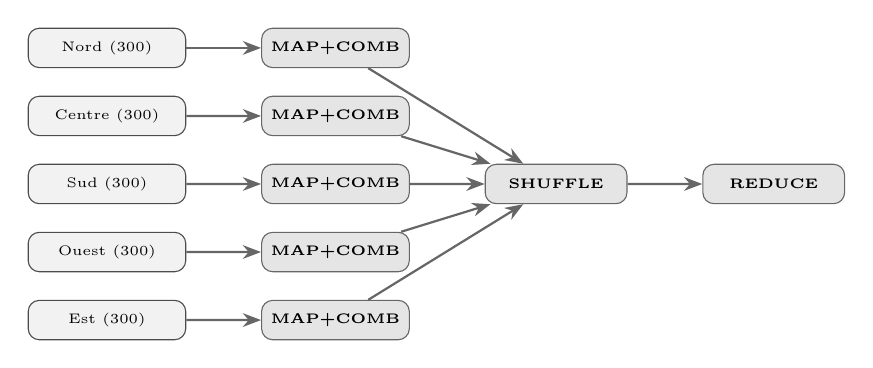
\begin{tikzpicture}[scale=0.9, node distance=0.35cm and 0.95cm,
  server/.style={draw=black!70, fill=black!5, rounded corners, minimum width=2cm, minimum height=0.5cm, font=\tiny},
  phase/.style={draw=black!60, fill=black!10, rounded corners, minimum width=1.8cm, minimum height=0.5cm, font=\tiny\bfseries},
  arrow/.style={-Stealth, thick, black!60},
]
  \node[server] (nord)   {Nord (300)};
  \node[server, below=of nord]   (centre) {Centre (300)};
  \node[server, below=of centre] (sud)    {Sud (300)};
  \node[server, below=of sud]    (ouest)  {Ouest (300)};
  \node[server, below=of ouest]  (est)    {Est (300)};

  \node[phase, right=0.95cm of nord]   (m1) {MAP+COMB};
  \node[phase, right=0.95cm of centre] (m2) {MAP+COMB};
  \node[phase, right=0.95cm of sud]    (m3) {MAP+COMB};
  \node[phase, right=0.95cm of ouest]  (m4) {MAP+COMB};
  \node[phase, right=0.95cm of est]    (m5) {MAP+COMB};

  \node[phase, right=0.95cm of m3] (sh) {SHUFFLE};
  \node[phase, right=0.95cm of sh] (red) {REDUCE};

  \foreach \s/\m in {nord/m1, centre/m2, sud/m3, ouest/m4, est/m5}
    \draw[arrow] (\s) -- (\m);
  \foreach \m in {m1,m2,m3,m4,m5}
    \draw[arrow] (\m) -- (sh);
  \draw[arrow] (sh) -- (red);
\end{tikzpicture}
\caption{Pipeline MapReduce : 5 serveurs en parallèle → Shuffle → Reducer}
\end{figure}

% ══════════════════════════════════════════════════════════════════════
%  3. LE PIPELINE MAPREDUCE
% ══════════════════════════════════════════════════════════════════════
\section{Le pipeline MapReduce appliqué au K-Means}

Une itération complète du K-Means MapReduce se déroule en trois phases enchaînées :
MAP+COMBINE (exécuté en parallèle sur chaque serveur), SHUFFLE (regroupement des
résultats) et REDUCE (calcul des nouveaux centroïdes). Ces phases se répètent jusqu'à
convergence.

\subsection{Phase MAP + COMBINE : calcul local sur chaque serveur}

La phase MAP est exécutée par un \textbf{mapper} sur chaque serveur régional.
Pour chaque capteur de son lot de données, le mapper calcule la distance
euclidienne aux $K$ centroïdes courants et assigne le capteur au cluster le plus proche.
Ce travail est effectué sur les données locales, sans communication inter-serveurs.

Le \textbf{Combiner} agrège ensuite localement les capteurs du même cluster :
au lieu de 300 enregistrements, chaque serveur envoie seulement $K$ sommes partielles
(somme des features + compteur). Ceci réduit le trafic réseau
d'un facteur $300/K = 100\times$ avec $K=3$.

\subsection{Phase SHUFFLE et REDUCE}

Le Shuffle regroupe les partiels par cluster. Le Reducer calcule ensuite le nouveau
centroïde de chaque cluster en combinant les sommes partielles :
\[
  c_k^{\text{new}} = \frac{\sum_w (\text{somme}_{w}^{(k)})}{\sum_w n_w^{(k)}}
\]
Cette opération est \textbf{mathématiquement exacte} et produit le même résultat que
l'algorithme séquentiel.

\subsection{Efficacité du Combiner}

Sans Combiner, chaque serveur transmettrait les $N$ enregistrements bruts de ses
capteurs, soit $N \times W = 300 \times 5 = 1\,500$ enregistrements au total.
Grâce au Combiner, chaque serveur n'envoie que $K$ sommes partielles, soit
$K \times W = 3 \times 5 = 15$ valeurs. Le trafic réseau est ainsi réduit d'un
facteur $N/K = 100$ à l'échelle de base. Pour le dataset de stress à 50\,000
capteurs au total ($\approx$10\,000 par partition selon le nombre de workers), ce facteur monte à $\approx 3\,333$, ce qui
illustre l'importance du Combiner à grande échelle.

\subsection{Initialisation K-Means++}

La qualité du clustering dépend du choix des centroïdes initiaux. L'implémentation
utilise l'heuristique \textbf{K-Means++} : le premier centroïde est choisi
aléatoirement, puis chaque centroïde suivant est sélectionné avec une probabilité
proportionnelle au carré de sa distance au centroïde existant le plus proche.
Cette stratégie réduit le risque de convergence vers des minima locaux et améliore
la qualité finale des clusters.


% ══════════════════════════════════════════════════════════════════════
%  4. IMPLÉMENTATION
% ══════════════════════════════════════════════════════════════════════
\section{Implémentation et résultats préliminaires}

\subsection{Organisation des modules}

Le pipeline est implémenté en Python avec une séparation claire des responsabilités.

\begin{center}
\small
\begin{tabular}{>{\ttfamily}l p{8.5cm}}
\toprule
\normalfont\textbf{Module} & \textbf{Responsabilités} \\
\midrule
\normalfont generate\_data.py & Génération des données IoT simulées : 5 serveurs
  régionaux, 300 capteurs/serveur, 3 profils de comportement + dataset stress 50k \\[2pt]
\normalfont utils.py       & Fonctions utilitaires partagées : distance euclidienne,
  normalisation z-score, SSE, K-Means++, chargement CSV \\[2pt]
\normalfont kmeans\_mr\_job.py & Cœur MapReduce : mapper-combiner, shuffle, reducer,
  orchestrateur d'itération, \texttt{multiprocessing.Pool} \\[2pt]
\normalfont kmeans\_mapreduce.py & Boucle itérative K-Means, critère de convergence,
  mode chunk et mode multi-serveurs \\[2pt]
\normalfont kmeans\_classic.py & K-Means séquentiel de référence, timeout configurable \\[2pt]
\normalfont benchmark.py & Benchmark comparatif en 3 phases (fichiers CSV, montée en charge, projections milliard) ; timeout 20\,s \\[2pt]
\normalfont simulation\_comparison.py & Montée en charge 10k–1M (dashboard) ou 1k–2M
  (complet) ; simulation réseau IoT 1\,Mbps ; timeout 15\,s en mode complet \\
\bottomrule
\end{tabular}
\end{center}

\noindent Chaque module a des dépendances minimales et peut être testé indépendamment.
L'architecture favorise la maintenabilité et l'extension future.

\subsection{Code du Mapper-Combiner et du Reducer}

Le code implémente directement les phases MAP, COMBINE et REDUCE décrites en
section~3. Le Mapper-Combiner s'exécute en parallèle via \texttt{multiprocessing.Pool}
sur les $W$ serveurs ; le Reducer s'exécute ensuite une seule fois pour produire
les nouveaux centroïdes.

\noindent\textbf{Détails d'implémentation :}
\begin{itemize}
\item Le mapper parcourt chaque capteur du chunk, calcule sa distance à chaque
  centroïde via la distance euclidienne, et l'assigne au cluster le plus proche.
\item Le combiner agrège les capteurs du même cluster en une seule entrée : somme
  des vecteurs de features et compteur d'éléments.
\item Le reducer reçoit toutes les sommes partielles d'un cluster et les combine
  pour calculer le centroïde final.
\item La convergence est vérifiée par la norme L2 entre centroïdes successifs :
  $\|c_k^{\text{old}} - c_k^{\text{new}}\|_2 < 10^{-4}$.
\end{itemize}

\begin{lstlisting}[caption={Mapper-Combiner et Reducer (kmeans\_mr\_job.py)},
                   language=Python, basicstyle=\scriptsize\ttfamily]
def mapper_combiner(args):   # called via Pool.map  (single tuple argument)
    chunk_lines, centroids = args
    partial = {}
    for line in chunk_lines:
        line = line.strip()
        if not line or line.startswith("sensor_id"):
            continue
        parts = line.split(",")
        try:
            point = [float(parts[i]) for i in FEATURE_INDICES]
        except (ValueError, IndexError):
            continue
        distances = [euclidean(point, c) for c in centroids]
        cluster_id = distances.index(min(distances))
        if cluster_id not in partial:
            partial[cluster_id] = ([0.0]*len(point), 0)
        s, cnt = partial[cluster_id]
        partial[cluster_id] = ([s[d]+point[d] for d in range(len(point))], cnt+1)
    return partial

def reducer(cluster_id, values):
    total_sum, total_count = None, 0
    for partial_sum, count in values:
        total_sum = (list(partial_sum) if total_sum is None
                     else [a+b for a,b in zip(total_sum, partial_sum)])
        total_count += count
    new_centroid = ([s/total_count for s in total_sum] if total_count > 0
                    else total_sum or [0.0]*4)
    return cluster_id, new_centroid, total_count
\end{lstlisting}

L'orchestrateur commence par soumettre les chunks aux workers via \texttt{Pool.map}.
Il collecte ensuite les résultats partiels et les regroupe par identifiant de cluster
(phase Shuffle). Enfin, il appelle le Reducer pour calculer les nouveaux centroïdes.
À chaque itération, la convergence est contrôlée par la condition
$\|c_k^{\text{old}} - c_k^{\text{new}}\|_2 < 10^{-4}$, ce qui garantit la stabilité
des résultats tout en limitant le nombre d'itérations nécessaires.


\subsection{Exemple concret : 6 capteurs sur 2 serveurs}

On considère 6 capteurs ($K{=}2$, features : température T et humidité H) sur 2 serveurs.
Centroïdes K-Means++ : $C_0{=}[34,78]$ (rural/chaud), $C_1{=}[22,44]$ (urbain).

\smallskip
\noindent\textbf{Itération 1 — MAP} : chaque serveur calcule $d{=}\sqrt{\Delta T^2+\Delta H^2}$ et affecte au plus proche.

\begin{center}
\small
\begin{tabular}{@{}ccrrc@{}}
\toprule
\textbf{Serv.} & \textbf{Capteur} & $d(\cdot,C_0)$ & $d(\cdot,C_1)$ & \textbf{Aff.} \\
\midrule
A & $S_1=[34,78]$ & 0.00 & 36.06 & $C_0$ \\
A & $S_2=[36,82]$ & 4.47 & 40.50 & $C_0$ \\
A & $S_3=[33,75]$ & 3.16 & 32.89 & $C_0$ \\
\midrule
B & $S_4=[21,42]$ & 38.28 & 2.24 & $C_1$ \\
B & $S_5=[23,48]$ & 31.95 & 4.12 & $C_1$ \\
B & $S_6=[22,44]$ & 36.06 & 0.00 & $C_1$ \\
\bottomrule
\end{tabular}
\end{center}

\noindent\textbf{COMBINE} : Srv.\,A émet $\{C_0:([34{+}36{+}33,\;78{+}82{+}75],\;3)\}{=}\{C_0:([103,235],3)\}$ ;
Srv.\,B émet $\{C_1:([21{+}23{+}22,\;42{+}48{+}44],\;3)\}{=}\{C_1:([66,134],3)\}$.
\textbf{2 émissions réseau} au lieu de 6 enregistrements bruts.

\noindent\textbf{SHUFFLE} : le Reducer reçoit $C_0{\leftarrow}([103,235],3)$ depuis A et
$C_1{\leftarrow}([66,134],3)$ depuis B.

\noindent\textbf{REDUCE} :
\[
  C_0^{\text{new}} = \tfrac{[103,235]}{3} = [34{,}33,\;78{,}33]
  \qquad
  C_1^{\text{new}} = \tfrac{[66,134]}{3} = [22{,}00,\;44{,}67]
\]
$\|C_0^{\text{new}}{-}C_0\| \approx 0{,}47 > 10^{-4}$ → non convergé ; itération 2 nécessaire.

\noindent\textbf{Itération 2} : les affectations sont inchangées → sommes partielles identiques
→ $\|\Delta C\|{=}0 < 10^{-4}$ : \textbf{convergé en 2 itérations.}

\noindent\textbf{Résultat final} : $C_0{=}\{S_1,S_2,S_3\}$ ($34{,}33\,\text{°C}$, $78{,}33\%$, rural) ;
$C_1{=}\{S_4,S_5,S_6\}$ ($22{,}00\,\text{°C}$, $44{,}67\%$, urbain).
Résultat \textbf{identique à l'algorithme classique} — l'agrégation par sommes partielles
est mathématiquement exacte. Gain réseau : $N/K{=}3$ ici, $100\times$ sur les données réelles.

% ══════════════════════════════════════════════════════════════════════
%  5. RÉSULTATS ET PERFORMANCES
% ══════════════════════════════════════════════════════════════════════
\section{Résultats et performances}

Cette section présente une évaluation comparative entre l'approche classique et MapReduce
selon trois axes : le temps d'exécution brut, la scalabilité face à la montée en charge,
et la qualité des clusters produits.

\subsection{Phase 1 — Benchmark sur fichiers CSV réels}

Les mesures ont été réalisées sur une machine à 4 CPU logiques, avec $K=3$ clusters,
un maximum de 10 itérations et un timeout de 20\,s (\texttt{benchmark.py}).

\begin{center}
\small
\begin{tabular}{lrrrp{3.8cm}}
\toprule
\textbf{Dataset} & \textbf{Points}
  & \textbf{Classique (s)} & \textbf{MapReduce (s)} & \textbf{Ratio} \\
\midrule
Normal         & 1\,500  & 0.072 & 0.125 & overhead 1.74$\times$ (pool de processus) \\
Stress test    & 50\,000 & 2.417 & 1.002 & \textbf{2.41$\times$ — plus rapide} \\
Multi-serveurs & 1\,500  & 0.071 & 0.141 & overhead 1.99$\times$ (normal à ce volume) \\
\bottomrule
\end{tabular}
\end{center}

\noindent\textbf{Observations :} Sur le petit dataset de 1\,500 capteurs, le surcoût
lié à la création du pool de processus est mesurable mais reste faible (environ 50\,ms).
En revanche, sur 50\,000 capteurs, le parallélisme devient clairement avantageux :
MapReduce atteint un speedup de $2.41\times$ ($2.417\,\text{s} / 1.002\,\text{s}$).

\subsection{Scalabilité — montée en charge et projections milliard}

Ces mesures portent sur des données synthétiques avec un timeout de 20\,s.
Les colonnes \textit{Classique (calcul)} et \textit{MapReduce (calcul)} indiquent
le \textbf{temps de calcul pur} pour chaque approche. La colonne \textit{Gain total réseau}
compare les temps \textbf{totaux} en y ajoutant le coût de transfert réseau : pour
l'approche classique, toutes les données brutes doivent transiter sur un lien IoT à
1\,Mbps ; pour MapReduce, seules 15 sommes partielles sont envoyées sur un LAN Gigabit.
Pour les lignes extrapolées (10M à 1G capteurs), la colonne \textit{Classique} affiche
directement le temps total (calcul\,+\,réseau).

\begin{center}
\small
\resizebox{\linewidth}{!}{%
\begin{tabular}{rrrl}
\toprule
\textbf{Capteurs} & \textbf{Classique (calcul)} & \textbf{MapReduce (calcul)} & \textbf{Gain total réseau} \\
\midrule
100\,000    & 3.978\,s  & 2.427\,s  & 29.6\,s vs 2.4\,s → \textbf{12.2$\times$} \\
500\,000    & \textbf{TIMEOUT} & 12.657\,s & $>$2\,min vs 12.7\,s → \textbf{11.7$\times$} \\
1\,000\,000 & \textbf{TIMEOUT} & 31.360\,s & $\approx$4.6\,min vs 31.4\,s → \textbf{8.8$\times$} \\
\midrule
\multicolumn{4}{l}{\textit{Extrapolation $O(n)$ — classique depuis 100k cap., MR depuis 1M cap. (réseau IoT 1\,Mbps)}} \\
\midrule
10\,000\,000     & $\approx$49\,min (total)   & $\approx$5\,min  & \textbf{9.4$\times$} \\
100\,000\,000    & $\approx$8.2\,h (total)    & $\approx$52\,min & \textbf{9.4$\times$} \\
1\,000\,000\,000 & \textbf{$\approx$3.4 jours}& $\approx$8.7\,h  & \textbf{9.4$\times$} \\
\bottomrule
\end{tabular}%
}
\end{center}

\noindent Le seuil critique se situe à \textbf{500\,000 capteurs}. En dessous de ce
seuil, l'approche classique reste utilisable ; au-delà, elle dépasse le timeout de 20\,s
alors que MapReduce converge en 12.657\,s. À l'échelle du milliard, l'écart devient
radical : rien que le transfert des données brutes (32\,Go à 1\,Mbps) mobilise le réseau
pendant environ 3 jours, avant même que le calcul puisse commencer. MapReduce, lui,
livre le résultat en $\approx$8,7\,h, soit un gain de $9{,}4\times$.

\subsection{Discussion des résultats}

\noindent\textbf{Overhead vs bénéfice :} À faible volume (1\,500 capteurs), la création du pool coûte
$\approx$50\,ms et génère un overhead. Dès 50\,000 capteurs cet overhead est amorti ($2.41\times$) ;
au-delà de 500\,000, l'approche classique dépasse le timeout et MapReduce devient la seule option.

\noindent\textbf{Impact réseau :} En contexte IoT réel à 1\,Mbps, dès 100\,000 capteurs le
transfert brut mobilise 25,6\,s tandis que MapReduce n'envoie que 15 sommes partielles
($<\!1\,\text{ms}$) : gain total $12.2\times$. Ce déséquilibre réseau devient dominant au milliard.

\subsection{Qualité des clusters produits}

Cette section vérifie que la parallélisation ne dégrade pas la qualité du clustering.
Nous comparons pour cela les centroïdes et la SSE obtenus par les deux approches sur
le dataset de référence de 1\,500 capteurs avec $K=3$ clusters.

\begin{center}
\small
\begin{tabular}{clrp{5cm}}
\toprule
\textbf{Cluster} & \textbf{Centroïde} & \textbf{Taille} & \textbf{Profil identifié} \\
\midrule
$C_0$ & [27.6°C, 59.3\%, 1.08\,m/s², 260\,kbps] & 524 &
  Suburbain : conditions intermédiaires \\[3pt]
$C_1$ & [34.3°C, 78.3\%, 0.53\,m/s², 124\,kbps] & 525 &
  Zone rurale/forestière : chaude, humide \\[3pt]
$C_2$ & [22.2°C, 45.2\%, 2.49\,m/s², 512\,kbps] & 451 &
  Urbain industriel : vibration, trafic élevés \\
\bottomrule
\end{tabular}
\end{center}

\noindent Les deux algorithmes produisent exactement la même somme des erreurs
quadratiques : $\text{SSE}_{\text{classique}} = \text{SSE}_{\text{MapReduce}} = 3\,550\,130.6$.
Les trois clusters identifiés correspondent à des profils IoT distincts et cohérents.
Ces résultats confirment que la parallélisation par MapReduce ne compromet en rien
la précision du clustering.


% ══════════════════════════════════════════════════════════════════════
%  6. CONCLUSION
% ══════════════════════════════════════════════════════════════════════
\section{Conclusion}

Ce travail a mis en œuvre et évalué le paradigme MapReduce pour le clustering K-Means
sur un réseau de capteurs IoT distribués. Cinq enseignements principaux se dégagent.

\begin{enumerate}

\item \textbf{Exactitude mathématique :} MapReduce produit exactement le même résultat
que l'algorithme classique : la SSE est identique ($3\,550\,130.6$), car l'agrégation
par sommes partielles est une transformation mathématiquement exacte.

\item \textbf{Seuil de rentabilité :} MapReduce devient avantageux dès \textbf{50\,000
capteurs} en calcul pur ($2.41\times$) et plus tôt encore en scénario IoT réel —
à 100\,000 capteurs, le gain total atteint déjà $12.2\times$.

\item \textbf{Efficacité réseau du Combiner :} En réduisant $N$ enregistrements à $K$
sommes partielles, le Combiner divise le trafic d'un facteur $N/K$, soit $\times 100$
à l'échelle de base et $\times 3\,333$ à 50\,000 capteurs au total.

\item \textbf{Seuil critique à 500\,000 capteurs :} Au-delà de ce seuil, l'algorithme
classique dépasse le timeout de 20\,s alors que MapReduce termine dans tous les cas
testés jusqu'à 1\,000\,000 capteurs (31.360\,s).

\item \textbf{Projection à l'échelle milliard :} À 1 milliard de capteurs, le classique
nécessite $\approx$3,4 jours contre $\approx$8,7\,h pour MapReduce ($9{,}4\times$) :
MapReduce \emph{termine} pendant que le classique \emph{collecte encore les données}.

\end{enumerate}

MapReduce pour K-Means offre ainsi exactitude, scalabilité et efficacité réseau,
avec un avantage qui s'amplifie à mesure que le volume de données croît.

\end{document}
